\chapter{Implementation}
\label{ch:concept_and_implementation}


This chapter describes the development of the Mixed Reality Environment, a platform designed to support RitL testing by combining simulation with AR projection and VR. The resulting system bridges the gap between purely digital simulations and real-world experiments by creating a common workspace where physical robots and virtual objects coexist and interact.

The central concept of this environment is the projection of a simulated world directly onto the laboratory floor. Rather than testing robots in completely physical setups or purely within software simulations, this system projects dynamic, physics-based elements into the real world. As can be seen from Figure~\ref{fig:mr_environment_overview}, the physical robot moves across the real floor while sensing and acting upon virtual objects. This projection has a dual purpose: it provides instant visual feedback to a human observer and enables the robot to receive sensor data that reflect the state of the virtual scene. This allows the robot to detect and respond to simulated entities as if they were physically present.
\begin{figure}[H]
\centering
\includegraphics[width=0.9\textwidth]{images/implemantion_intro.jpg} % Placeholder for your figure
\caption{The Mixed Reality Environment in operation. The physical robot interacts with a projected Smart Farming scenario, where the robot and the digital twin are synchronized via ROS~2.}
\label{fig:mr_environment_overview}
\end{figure}

To enable these applications, the system integrates several key functions into an architecture to realize the Mixed Reality Environment. First, it maintains a digital twin of the robot. This digital twin is synchronized with the movement of the physical hardware but can interact with the simulation's physics engine. This allows for complex actions, such as pushing virtual boxes or colliding with moving objects. This ensures that the simulation responds realistically to the robot's physical presence rather than serving as a static background.

In addition to maintaining a digital twin, the system also simulates sensors for the robot. It generates virtual LiDAR scans and camera images from the robot's perspective, allowing robotic applications to receive virtual sensor data. This enables thorough testing of navigation and vision algorithms within the mixed reality environment.

The architecture uses ROS~2~\cite{MFG22} as the primary communication backbone. By integrating ROS~2 nodes directly into the simulation engine, the virtual environment acts as a first-party participant in the robot's network. It manages time synchronization to prevent timing-related errors, handles the loading of different scenarios and provides two-way exchange of status data and control commands.

Besides sensor simulation, the environment also supports real-time diagnostic feedback. The system functions as a monitoring tool by projecting the robot's internal operating data back onto the physical workspace and the VR interface. Performance metrics, such as temperature, Random Access Memory (RAM) usage, and location coordinates, are shown on information panels attached to the digital twin in the 3D environment. Moreover, the system shows the robot's live camera feed within the virtual scene. This allows operators to observe the robot's physical behavior alongside its internal status and visual perception in real time.

The platform provides an adaptable and scalable testing solution by integrating physics, sensor simulation, and autonomous control logic into a synchronized mixed reality environment. The only factor limiting the test environment's complexity is software, not its physical design. The technological decisions, system architecture, and particular implementation of these elements will be covered in detail in the sections that follow.

\section{Comparative Analysis}
The simulation engines that were considered as candidates to implement the Mixed Reality Environment are: Gazebo~\cite{Gazebo}, Isaac Sim~\cite{IsaacSim}, Unreal Engine~\cite{unrealengine}, and Unity~\cite{Uni23}. All were evaluated based on five critical criteria: visual fidelity, physics capabilities, learning curve, community support, and native integration with VR, AR, and ROS~2. Table~\ref{tab:sim_comparison} summarizes the results of this evaluation.

\begin{table}[H]
    \centering
    \caption{Comparison of Simulation Engines for Mixed Reality Digital Twins~\cite{Gonzalez2025, Kargar2024, Singh2025, Coronado2023}.}
    \label{tab:sim_comparison}
    \begin{tabularx}{\textwidth}{@{}lXXXX@{}}
        \toprule
        \textbf{Feature} & \textbf{Gazebo} & \textbf{Isaac Sim} & \textbf{Unreal Engine} & \textbf{Unity} \\ 
        \midrule
        \textbf{Primary Use} & Control \& Navigation & AI \& Photorealism & Photorealism & HRI \& MR (VR/AR) \\ 
        \textbf{Visual Fidelity} & Moderate & Very High & Very High & High \\ 
        \textbf{Physics Engine} & ODE / Bullet & PhysX 5 & Chaos / PhysX & PhysX \\ 
        \textbf{Learning Curve} & Steep & Advanced & Steep (C++) & Moderate (C\#) \\ 
        \textbf{Community} & High (ROS) & Moderate & High (Gaming) & Very High (MR) \\ 
        \textbf{ROS~2 Integ.} & Native & Bridge & Bridge & Plugin (Native) \\ 
        \textbf{Hardware} & Low & Very High (RTX) & High & Moderate \\ 
        \bottomrule
    \end{tabularx}
\end{table}

\subsection{Selection Rationale}
Based on the comparative analysis, the Unity Engine was selected as the implementation platform for this thesis. This decision is driven by four key factors that align with the system requirements:

\begin{itemize}
    \item \textbf{VR Framework} (\hyperref[req:FR-03]{FR-03}): Unity has an integrated framework for VR applications~\cite{Coronado2023}. In contrast, simulators like Gazebo lack native VR support, which is critical for the proposed human-robot interaction interface.
    
    \item \textbf{Visual Fidelity \& Physics} (\hyperref[req:FR-01]{FR-01}, \hyperref[req:FR-02]{FR-02}): Unity provides high-fidelity visualization alongside PhysX integration. This offers an optimal balance between performance and visual quality, avoiding the restrictive hardware requirements associated with NVIDIA Isaac Sim~\cite{Gonzalez2025}.
    
    \item \textbf{Development Efficiency}: The use of C\# scripting, combined with documentation and community support, makes Unity more accessible for rapid prototyping than the C++ environment of Unreal Engine~\cite{Coronado2023}.

    \item \textbf{ROS~2 Integration} (\hyperref[req:FR-04]{FR-04}): The availability of the \texttt{Ros2ForUnity}~\cite{Rob24} asset enables the simulation to function as a first-party participant in the ROS~2 network. This means it supports the low-latency communication requirement by avoiding external bridge applications.
\end{itemize}





\section{System Architecture}
\label{sec:system_architecture}

The realization of the Mixed Reality Environment requires a distributed software architecture that connects the rendering capabilities of the Unity engine with real-time robotic control. The system is designed to satisfy the requirement for Middleware Integration (\hyperref[req:FR-04]{FR-04}) by establishing a unified communication layer between the simulation host and the robotic applications using ROS~2.

\subsection{Hardware and Software Topology}
\label{subsec:hardware_topology}

To ensure high performance and support for specific hardware peripherals, the system topology is consolidated into a single workstation acting as the central server, supported by distributed wireless clients. As shown in Figure~\ref{fig:hardware_topology}, the architecture is divided into four distinct computational domains:

\begin{enumerate}
    \item \textbf{Workstation (Windows 11 Host):} The primary host runs Windows 11 to support the Unity Engine and the ALVR (Air Light VR) Server~\cite{ALVR_Github} natively. This layer manages the physics engine and renders the digital twin and its virtual environment. It physically interfaces with the visual peripherals: a ceiling-mounted Projector via HDMI for floor projection and an Overhead Tracking Camera via USB to provide localization data.
    
    \item \textbf{Control Environment (WSL 2):} The computationally intensive robotic software runs on Ubuntu 24.04 within the Windows Subsystem for Linux (WSL) on the same workstation. This isolation allows the \textit{Nav2 Stack}, \textit{Robotic Applications Logic} and the \textit{ArUco Tracking System} to run in a native Linux environment while communicating with the Windows host via a low-latency Localhost connection.
    
    \item \textbf{Physical Robot (EMAROs):} The mobile robot\cite{EMAROs_Ref} operates as an independent node running Ubuntu 24.04 and ROS~2~Jazzy Jalisco. The onboard software is launched by the \texttt{emaros\_launch} package, which manages hardware drivers for motor controllers and sensors. It connects to the system wirelessly via Wi-Fi.

    \item \textbf{VR Interface (Meta Quest Pro):} The VR headset functions as a standalone client running Meta Horizon OS. It executes the ALVR Client~\cite{ALVR_Github} application, which is responsible for decoding the incoming video stream and handling spatial input.
\end{enumerate}

\begin{figure}[H]
    \centering
    \includegraphics[width=0.65\textwidth]{images/hardware_topology.png}
    \caption{The Hardware and Software Topology of the Mixed Reality Environment.}
    \label{fig:hardware_topology}
\end{figure}

The VR integration (\hyperref[req:FR-16]{FR-16}) relies on ALVR, an open-source remote rendering solution that splits the computational workload. The ALVR Server, running on the workstation, captures the rendered frames from Unity and encodes them into a high-bitrate video stream. This stream is transmitted via Wi-Fi to the ALVR Client on the Meta Quest Pro. The headset decodes and displays this video feed while simultaneously capturing head-tracking data and controller inputs, which are transmitted back to the server.~\cite{ALVR_Github}

The network infrastructure is centered around a dedicated Router. The workstation is connected via Ethernet, while the EMAROs robot and Meta Quest Pro connect via Wi-Fi. This topology ensures that latency-sensitive traffic, such as the ALVR video stream and ROS~2 control commands, faces minimal interference.


\subsection{Software Component Architecture}
\label{subsec:software_components}

The software architecture follows a modular publisher-subscriber pattern. To integrate the Unity game engine with the robotic network, the system utilizes the \texttt{ROS2ForUnity}~\cite{RFU24} library (\hyperref[req:FR-04]{FR-04}).

To facilitate modularity~(\hyperref[req:NFR-03]{NFR-03}), the implementation relies on Unity's component-based architecture. In this framework, entities within the simulation, such as the robot or the environment, are represented as \texttt{GameObjects}. These objects function as containers that hold various functional modules known as \textit{components}. By inheriting from Unity's base class \texttt{MonoBehaviour}, C\# scripts gain access to the engine's event lifecycle. This allows them to be attached to \texttt{GameObjects} and execute logic in response to specific engine events, such as frame updates or physics steps.

The core of the network integration is the \texttt{ROS2UnityComponent}~\cite{RFU24} class. This component acts as a wrapper around the standard ROS~2 middleware. Inheriting from \texttt{MonoBehaviour}, it must be attached to a \texttt{GameObject} in the scene to function. Upon startup, this component initializes the ROS~2 context, ensures that a valid connection is established and handles the lifecycle of the ROS~2 nodes running within the simulation. It allows other scripts to access the ROS~2 network by referencing this central component to create publishers, subscribers, and service clients.

The functionality of the digital twin is driven by such scripts that interact with the engine's internal state machine. To guarantee that the physical simulation remains deterministic while visualization remains smooth, the architecture uses specific phases of the Unity execution loop~\cite{UnityDocumentation}:

\begin{itemize}
    \item \textbf{Initialization (\texttt{Start}):} This method is called once when the script is first enabled, before any frames are updated. In this architecture, it is used to retrieve the reference to the \texttt{ROS2UnityComponent}~\cite{RFU24}, initialize the specific ROS~2 nodes, and set up the necessary publishers and subscribers.
    
    \item \textbf{Physics Loop (\texttt{FixedUpdate}):} This method executes at a constant, user-defined time step, independent of the visual frame rate. All physics-based calculations, such as updating the robot's position based on received velocity commands or handling collision detection, occur in this loop. This ensures that the robot's physical behavior is consistent regardless of graphical performance.
    
    \item \textbf{Rendering Loop (\texttt{Update}):} This method runs once every frame. It is utilized for logic that is not physics-related, like updating UI elements, rendering diagnostic lines, or capturing camera frames for visualization. This separation ensures that high-frequency visual updates do not interfere with the stability of the physics engine.
\end{itemize}

Figure~\ref{fig:software_architecture} provides an overview of how these Unity scripts interact with the external ROS~2 nodes via topics. Detailed descriptions of these components follow in Sections \hyperref[sec:robot_representation_and_control]{4.3.} and \hyperref[sec:environmental_simulation_capabilities]{4.4.}

\begin{figure}[H]
    \centering
    % TODO: Create a diagram showing:
    % Left side: Unity Components (LidarSensor, CameraSensor, VirtualRobotController).
    % Middle: Arrows representing ROS Topics (/scan, /camera/image, /cmd_vel).
    % Right side: ROS Nodes (Nav2 Stack, Perception Node, Mission State Machine).
    \includegraphics[width=1.0\textwidth]{images/software_architecture.png} 
    \caption{Software Component Architecture. Unity scripts act as ROS~2 nodes, publishing sensor data and subscribing to control commands using ROS~2 topics.}
    \label{fig:software_architecture}
\end{figure} % 

\subsection{Time Synchronization}
\label{subsec:time_sync}

A critical challenge in Robot-in-the-Loop testing is how to synchronize time between the simulation and the robot's software. If the simulation runs slower or faster than real-time, the navigation algorithms of the robot may calculate velocities that are incorrect. To fulfill the requirement for Time Synchronization (\hyperref[req:FR-05]{FR-05}), the system decouples the ROS network from the computer's system time.

The \texttt{ClockPublisher.cs} script in Unity acts as the master clock. It calculates the time since the start of the simulation and publishes it to the \texttt{/clock} topic. The ROS~2 nodes running on the workstation, such as the navigation stack, are configured with \texttt{use\_sim\_time = true}, forcing them to synchronize their logic with the Unity engine.

To ensure consistency, a \texttt{RosTimeHelper.cs} utility is used by all ROS~2 publishers in the Unity scripts. This script ensures that data leaving Unity is stamped with the exact simulation time of the frame it was created in to prevent data drift.



\section{Robot Representation and Control}
\label{sec:robot_representation_and_control}
The robot in the Mixed Reality Environment runs in one of two modes: either as a completely simulated virtual robot or as a synchronized digital twin of the physical EMAROs~\cite{EMAROs_Ref} platform. To ensure consistency, both of these modes use the same visual and geometric model. This model is a simple cylinder that approximates the physical size of the robot for collision detection while keeping computational costs low. The behavior of this cylinder depends on the active control script, allowing the system to switch between physics-based simulation and position-based synchronization based on the requirements of the test. To select the desired mode, the user can enable in the Unity Editor either the model of the digital twin or the purely virtual robot.

\subsection{The Purely Virtual Robot}
In the standalone simulation mode, the robot is controlled by the \texttt{Virtual\-Robot\-Controller.cs} (\hyperref[req:FR-09]{FR-09}). This component allows for the validation of high-level control logic in a safe environment before it is deployed on real hardware. Unlike simulations that teleport a robot to a target point, this implementation uses the Unity physics engine PhysX to simulate realistic movement.

The controller acts as a ROS~2 node that accepts velocity commands (\texttt{cmd\_vel}) and publishes odometry data. To handle data exchange between the asynchronous ROS~2 thread and the Unity main thread, incoming commands are buffered in a thread-safe \texttt{ConcurrentQueue}. During the physics step of Unity (\texttt{FixedUpdate}), the controller retrieves the latest command and applies it to the \texttt{Rigidbody} of the robot.

The script does not directly change the position of the robot. Instead, it modifies the velocity of the physics body. By applying limits to acceleration, the system simulates mass and inertia for the robot. The robot can push lightweight virtual objects, but heavy obstacles or walls will stop its movement. This provides realistic feedback to the navigation system.

Simultaneously, the controller provides ground truth data. It tracks the movement of the robot in Unity, converts the coordinates to the ROS~2 standard~\cite{MFG22} and publishes a timestamped odometry and tf messages (\hyperref[req:FR-10]{FR-10}). This closes the control loop for the external navigation logic.

\subsection{The Digital Twin Implementation}
When operating in RitL mode, the \texttt{PoseRobotController.cs} takes control. In this configuration, the virtual robot stops acting as a dynamic entity and instead becomes a digital twin of the real EMAROs~\cite{EMAROs_Ref} robot (\hyperref[req:FR-07]{FR-07}).

The controller listens to a pose topic given by the external ArUco tracking~\cite{JuliaBA} to move the digital twin. The incoming pose is provided in pixel coordinates from the tracking camera. It must be mapped onto the defined virtual area. On every new incoming pose, the script converts the pixel coordinates into Unity world space. To ensure alignment, an offset parameter enables the operator to perform a calibration of the digital twin so that its center is aligned with the physical mounting position of the tracking marker. The script republishes the synchronized pose as odometry and tf messages (\hyperref[req:FR-10]{FR-10}).

Unlike the purely virtual robot, the digital twin overrides the physics engine. It is set to a kinematic state, meaning it is immune to virtual forces. If the physical robot moves, the digital twin moves with it, ignoring virtual barriers. This allows the physical robot to push virtual objects with absolute force. This way, the state of the virtual world always reflects physical reality.

\subsection{Safety and Failsafe Mechanisms}
A major challenge in mixed reality testing is signal latency or loss. If the physical robot leaves the tracking area or if the ArUco marker is blocked, position updates will stop. Without a failsafe, the digital twin would freeze while the physical robot continues to move blindly, causing a mismatch between reality and simulation.

To prevent this, the \texttt{PoseRobotController.cs} implements a safety watchdog  (\hyperref[req:FR-08]{FR-08}). The system continuously checks how long it has been since receiving the last pose update. If this delay exceeds a given safety limit, the system assumes tracking has been lost.

When this occurs, the controller marks the tracking state as invalid. Although the digital twin will stop moving in the simulation, the physical Robot might continue moving. For this reason, the system is designed to send a stop command over the \texttt{cmd\_vel} topic to the motors of the physical robot. This ensures the robot does not perform actions without simulation guidance. Once the tracking system re-acquires the robot, the watchdog resets and the digital twin resumes synchronization immediately.

\section{Environmental Simulation Capabilities}
\label{sec:environmental_simulation_capabilities}

To serve as an effective testbed for robotic applications, the virtual environment provides a dynamic and interactive simulation context. It incorporates the capability to manipulate objects physically, generate realistic sensor data and modify the state of the environment persistently. This section describes the implementation of these features, fulfilling the requirements for Sensor Simulation (\hyperref[req:FR-11]{FR-11}), Dynamic Environment Interaction (\hyperref[req:FR-13]{FR-13}), and the Command Interface (\hyperref[req:FR-12]{FR-12}).
\subsection{Physics-Based Interaction}

A key feature of the system is the robot's ability to physically connect with environmental objects. To achieve a rigid and predictable connection between the robot and manipulated items, the architecture uses a kinematic attachment method managed by the \texttt{AttachmentCommandManager.cs} and the \texttt{RobotAttachmentController.cs}.

ROS~2 command and control (\hyperref[req:FR-12]{FR-12}) is provided via the \texttt{/robot\_command} topic. Commands are sent as simple string messages (e.g., \texttt{"attach,plow"} or \texttt{"detach"}). It offers a single, consistent interface for the high-level robotic applications to request simulation state changes. The Command Manager runs on the Unity main thread and processes incoming entries from a thread-safe queue. On receiving an attach request, it searches for valid targets within a configurable radius using \texttt{Physics.OverlapSphere}.

When a valid target is identified, the system attaches it to the robot, as illustrated in Figure~\ref{fig:attachment_logic}. In Unity, the object is attached as a child of the robot's transform hierarchy at a specific mount point. Crucially, the system modifies the physics state of the attached object (\hyperref[req:FR-13]{FR-13}). Upon attachment, the script sets the object's \texttt{Rigidbody.isKinematic} property to true. This removes the object from the physics engine's dynamic calculations. This state change grants the robot's transform absolute authority over the object's position, eliminating any relative motion, jitter, or drift between the robot and the load during transport.

At the same time, the controller disables collisions between the robot and the tool using \texttt{Physics.IgnoreCollision}. Without this step, snapping the object to the robot would cause their geometries to overlap. The physics engine would attempt to separate them forcibly, potentially causing the equipment to be ejected unpredictably.

\begin{figure}[H]
    \centering
    % Left Image (Detached)
    \begin{minipage}{0.49\textwidth}
        \centering
        \includegraphics[width=\linewidth]{images/Detached.png} % Make sure extension is .png or .jpg
        \par\vspace{5pt} % Small gap between image and text
        (a) Detached State
    \end{minipage}%
    \hfill % Spacer
    % Right Image (Attached)
    \begin{minipage}{0.49\textwidth}
        \centering
        \includegraphics[width=\linewidth]{images/Attached.png} % Make sure extension is .png or .jpg
        \par\vspace{5pt}
        (b) Attached State
    \end{minipage}
    \caption{The robot attachment logic. (a) The robot approaches the target object.\\ (b) The object is kinematically coupled to the robot chassis.}
    \label{fig:attachment_logic}
\end{figure}

\subsection{Surface Modification}
To fulfill the requirement for dynamic environment interaction regarding surface textures (\hyperref[req:FR-13]{FR-13}), the system implements a modification mechanism. 

The modification logic relies on physics raycasting to identify the coordinates of the surface at the point of contact. When a valid hit is detected on the target surface, the \texttt{TrackPainter.cs}, which is attached to the robot model, calculates the pixel coordinates on the texture map. It then modifies the pixel buffer directly using \texttt{SetPixels32}, allowing the robot to paint on the ground as visible in Figure~\ref{fig:texture_painting}, changing the color to a configured color and thickness. These changes are committed to the GPU using the \texttt{Apply} method. In complex scenarios, multiple robotic applications (e.g., the robot, a VR controller, or a mouse interface) may attempt to modify the terrain simultaneously. To manage this, the \texttt{SharedPaintTextureRegistry.cs} functions as a singleton manager. It maintains a dictionary of active textures and guarantees that all painters operate on a single, shared instance of the \texttt{Texture2D}. This prevents race conditions where one application or user overwrites the work of another and guarantees data consistency across the simulation.

\begin{figure}[H]
    \centering
    \includegraphics[width=0.8\textwidth]{images/texture_painting.png}
    \caption{Demonstration of dynamic surface modification. The robot uses the \texttt{TrackPainter.cs} component to modify the floor texture in real time based on its trajectory, creating a persistent black trail.}
    \label{fig:texture_painting}
\end{figure}

\subsection{Sensor Simulation}
To validate the perception algorithms of the robotic applications, the system provides simulated sensors capable of generating video feed and ranging data (\hyperref[req:FR-11]{FR-11}).

The \texttt{LidarSensor.cs} component simulates a 2D planar laser scanner, as illustrated in Figure~\ref{fig:lidar_raycasting}, which can be attached to the virtual model of the robot. This implementation utilizes the Unity physics engine's raycasting API to query the scene geometry. In every simulation step, the component executes a loop corresponding to the configured number of beams. For each beam, the system calculates a direction vector based on the scan angle.

For each beam a \texttt{Physics.Raycast} is cast along the computed direction. If the ray intersects a collider on the configured collision layer, its hit distance is recorded. Otherwise, the beam is reported as an infinite range. The collected distances are packaged into a standard \texttt{sensor\_msgs/LaserScan} message. Immediately after the raycast loop finishes, the message is stamped with the current simulation time from the \texttt{ClockPublisher.cs} and published. This exact timestamping preserves temporal alignment with the navigation stack and prevents the ROS~2 transform (TF) system from rejecting the scan due to extrapolation errors caused by unsynchronized timestamps.
\begin{figure}[H]
    \centering
    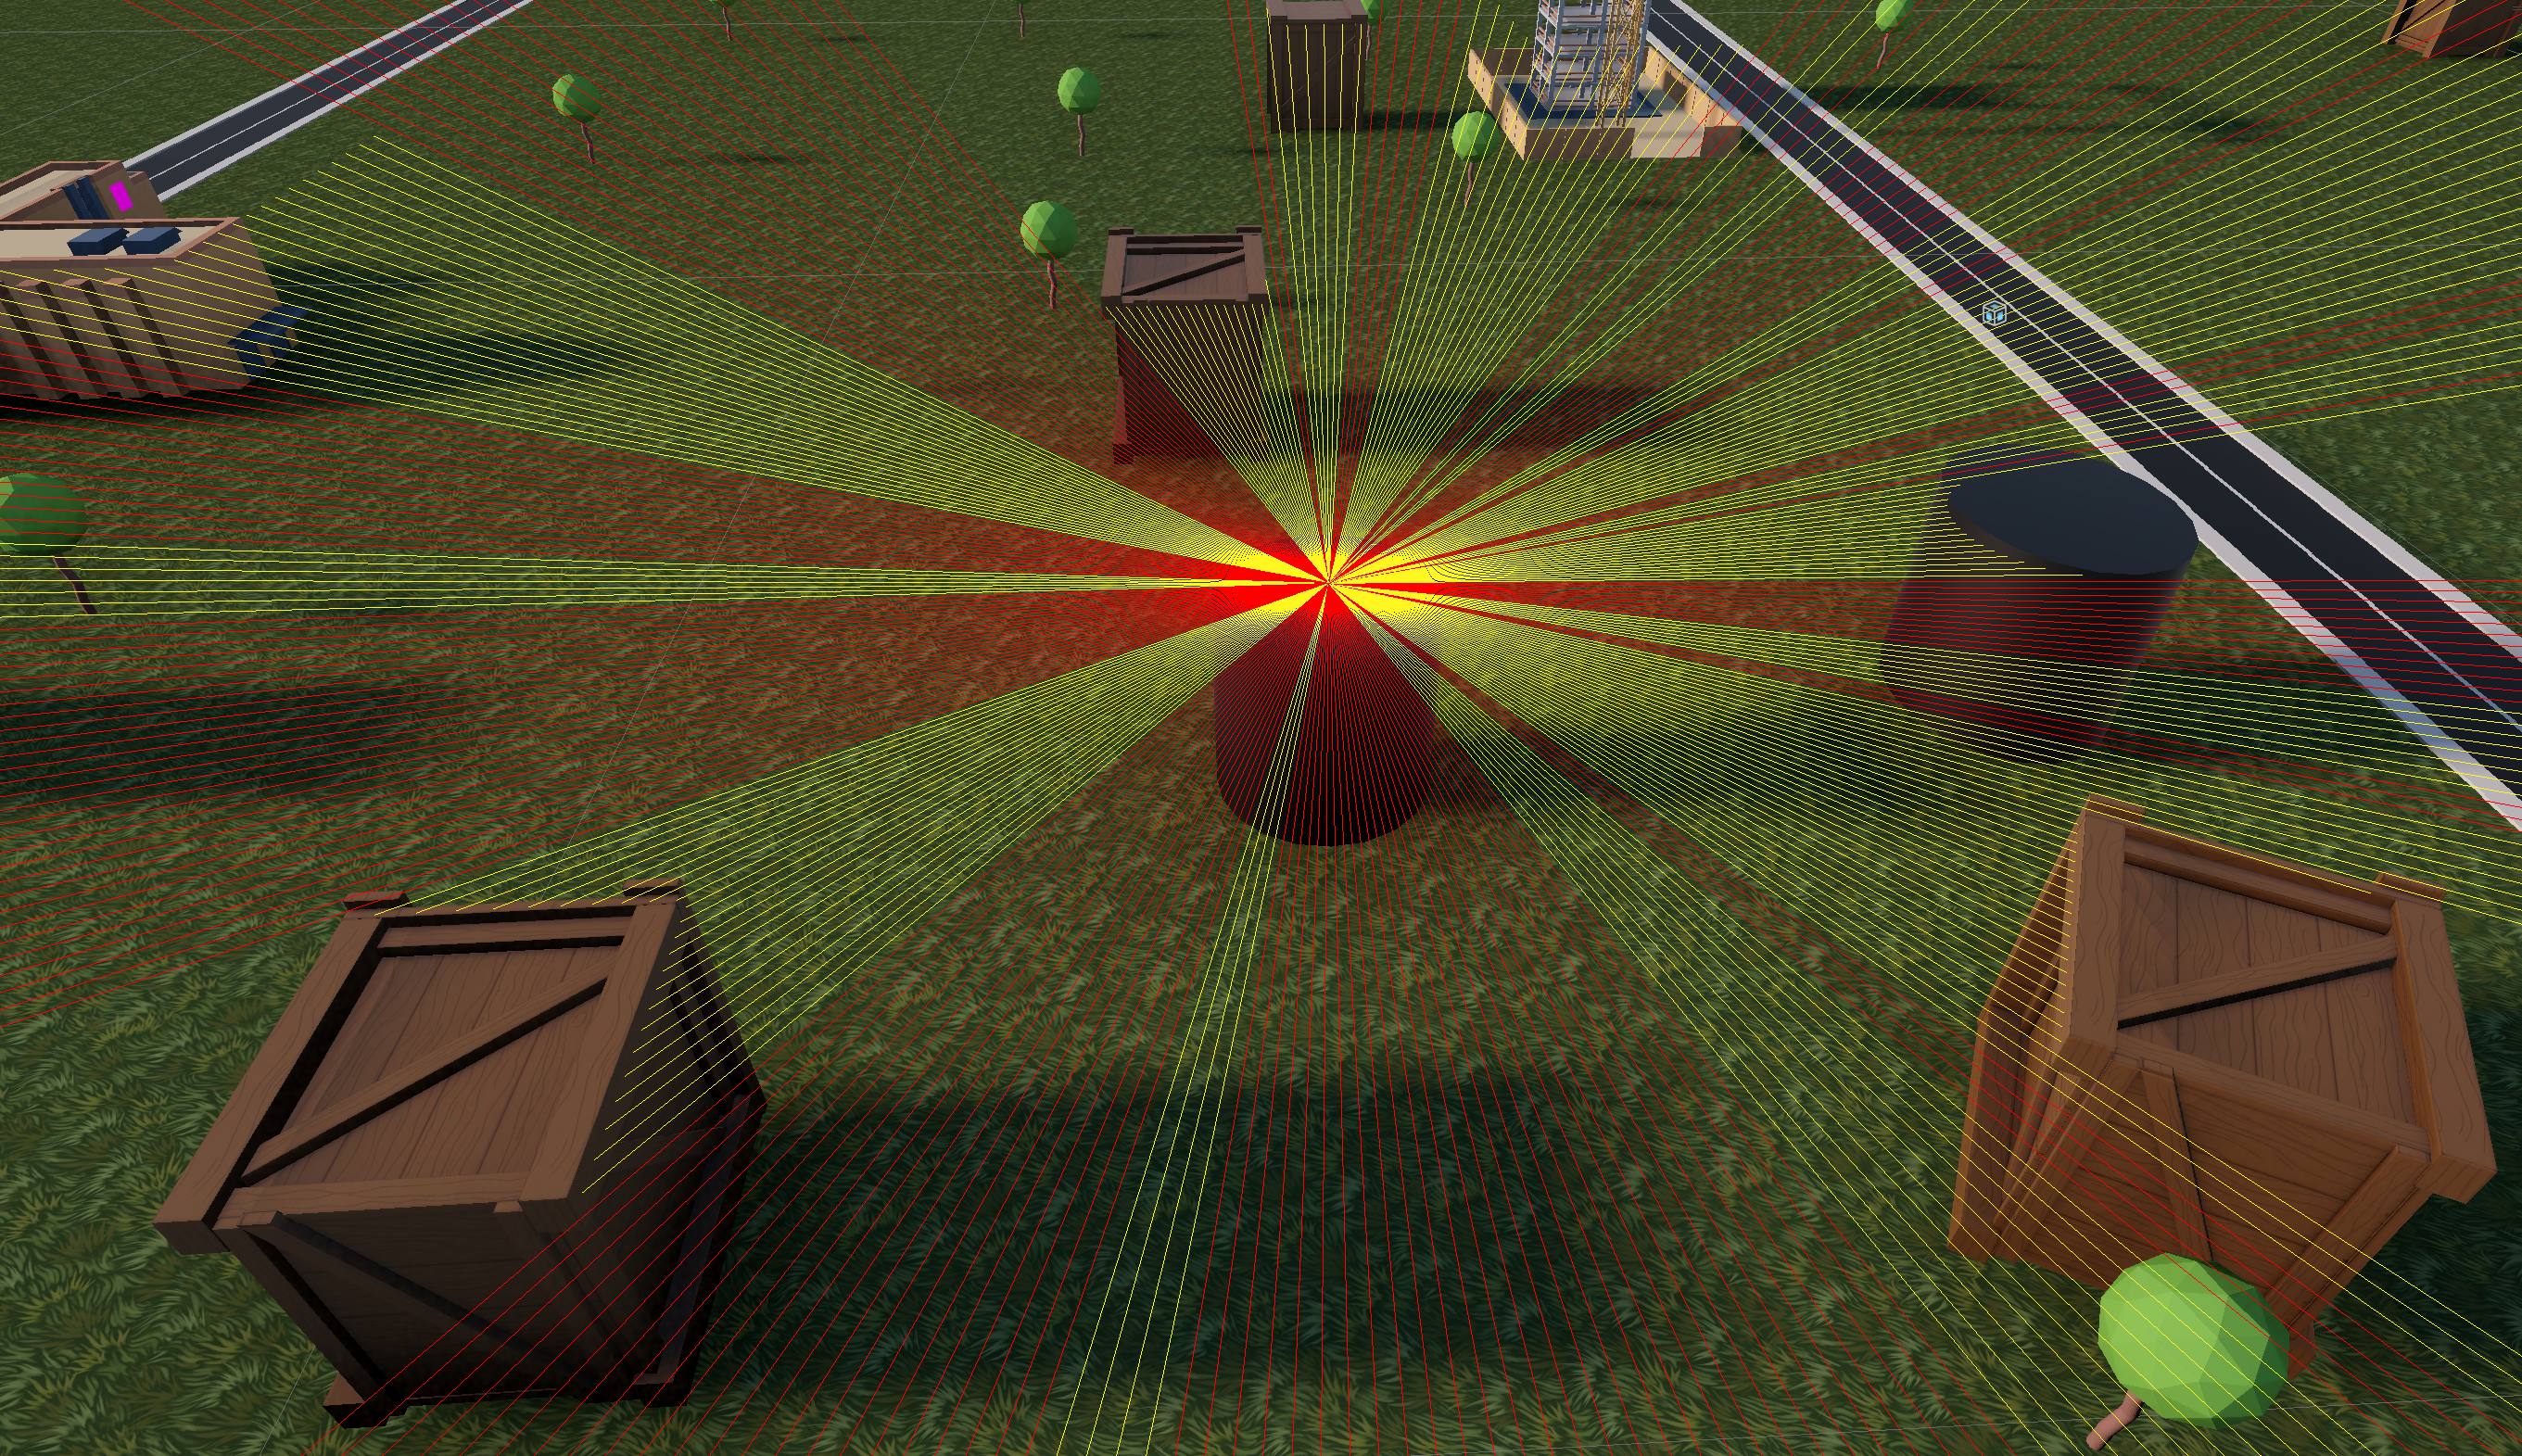
\includegraphics[width=0.8\textwidth]{images/lidar_raycast.png}
    \caption{Visualization of the LiDAR simulation in the editor. Red debug lines indicate raycasts that did not hit an obstacle within range, while yellow debug lines indicate valid hits registered by the physics engine.}
    \label{fig:lidar_raycasting}
\end{figure}

Visual perception is handled by the \texttt{CameraSensor.cs} component. This script attaches a dedicated Unity Camera to the robot model, which is configured to render the scene into a \texttt{RenderTexture} rather than the user's screen. This allows the simulation to generate visual data at a resolution independent of the application window.

The data extraction pipeline transfers the raw pixel data from the Graphics Processing Unit (GPU) memory to the Central Processing Unit (CPU) memory. Once on the CPU, the data is encoded into the appropriate format (e.g., raw RGB8 or JPEG) and published as a \texttt{sensor\_msgs/Image} or \texttt{CompressedImage}. To initialize the sensor, the \texttt{RobotCameraManager} instantiates the camera prefab at runtime and attaches it to the defined mount point in the robot hierarchy.


\subsection{Scenario and Object Management}
To support the requirement for \textbf{Scenario Management} (\hyperref[req:FR-06]{FR-06}), the architecture allows the system to switch between different test environments without restarting the entire application.

This is handled by the \texttt{SceneManager.cs} script. When it receives a command via the \texttt{/vera/load\_scenario} topic, it performs a clean reset sequence:
\begin{enumerate}
    \item \textbf{Shutdown:} The active ROS~2 connections are terminated. This ensures that all Unity nodes are properly removed from the network, preventing any lingering nodes from publishing outdated or invalid data.
    \item \textbf{Load:} Unity loads the new environment scene asynchronously.
    \item \textbf{Restart:} A fresh \texttt{ROS2UnityComponent}~\cite{RFU24} initializes, creating a new connection for the loaded scenario.
\end{enumerate}
This fresh start approach ensures that Unity components specific to one scenario do not interfere with others.


Beyond static geometry, the environment must support the lifecycle management of transient entities, such as the delivery boxes in the Logistics scenario. This is handled by the \texttt{DynamicObjectManager.cs}, which acts as a bridge between the ROS~2 data stream and the Unity instantiation engine (\hyperref[req:FR-13]{FR-13}).

The manager subscribes to the \texttt{/vera/virtual\_objects} topic, processing a custom message structure that defines an object's ID, type, and pose. Internally, the system maintains a dictionary mapping string identifiers to Unity Prefabs.
When an \texttt{ADD} or \texttt{MODIFY} command is received, the system checks if the object already exists. If it is new, the corresponding prefab is instantiated into the scene. If it exists, its transform is updated. This component handles the coordinate conversion between the two systems, mapping the right-handed ROS~2 position and orientation to the left-handed Unity world space. This allows external scripts or test runners to populate the scene with obstacles dynamically.

\section{Mixed Reality and User Interaction}
\label{sec:mixed_reality_and_user_interaction}

A primary objective of the framework is to enhance the transparency of the robotic system by providing intuitive, real-time feedback to human operators. This is achieved through an MR interface that visualizes internal robot states and allows for direct environmental manipulation. This section details the implementation of augmented telemetry, sensor projection and interactive control systems designed for both desktop and VR contexts.

\subsection{Environment Projection}
\label{subsec:environment_projection}

To fulfill the requirement for a 1:1 Augmented Reality projection (\hyperref[req:FR-15]{FR-15}), the system utilizes a dedicated Unity camera component configured to \texttt{orthographic}~\cite{UnityDocumentation}. Unlike perspective cameras, the orthographic view preserves parallel lines and consistent object scales regardless of their distance from the camera~\cite{UnityDocumentation}. This property is essential for projecting a map that aligns physically with the flat laboratory floor.

The camera is positioned at a fixed height looking downward. The alignment with the physical floor is achieved by calculating the exact \texttt{orthographicSize} parameter, which determines the vertical half-extent of the camera's viewing volume in world units~\cite{UnityDocumentation}. By mapping the pixel resolution of the projector to the metric dimensions of the projection area, as illustrated in Figure~\ref{fig:projection_mapping}, the system ensures that one unit in the simulation corresponds exactly to one meter on the physical floor.

\begin{figure}[H]
    \centering
    % TODO: Replace with the actual schematic image file
    \includegraphics[width=0.9\textwidth]{images/projection_mapping.png} 
    \caption{Schematic of the Environment Projection logic. The Unity Orthographic Camera (left) is calibrated such that its \texttt{orthographicSize} corresponds exactly to half the physical height of the projection area on the laboratory floor (right), ensuring a 1:1 metric scale.}
    \label{fig:projection_mapping}
\end{figure}

To display this view on the physical floor, the ceiling-mounted projector acts as a secondary monitor for the workstation. During operation, the \textit{Game View} window within the Unity Editor is undocked, moved to the projector's screen space and maximized to fill the projection area.
\subsection{Augmented Telemetry and Diagnosis}

To fulfill the Telemetry Display requirement (\hyperref[req:FR-14]{FR-14}), the system implements the \texttt{RobotInfoBillboard.cs} component. This script serves as a central data aggregator, establishing ROS~2 subscriptions based on a configurable list of topic definitions. It processes diverse message types and utilizes regular expressions to extract specific metrics, such as CPU and RAM usage, from text payloads.

For visualization in standard desktop views and AR projections, the system employs Unity's immediate mode Graphical User Interface (GUI) (\texttt{OnGUI}). The script calculates the screen-space coordinates of the robot's anchor using \texttt{Camera.WorldToScreenPoint} and applies rotational matrices to align the text. This ensures that the interface remains legible and strictly aligned with the screen plane, creating a floating overlay locked to the robot's position, as illustrated in Figure~\ref{fig:augmented_telemetry}.

In contrast, screen-space rendering is unsuitable for Virtual Reality due to depth perception issues. To address this, the architecture supports a World Space Canvas for VR users. In this configuration, textual information is rendered onto a 3D plane floating physically above the digital twin. To ensure readability from any perspective, the canvas implements a constraint that continuously orients the UI to face the VR headset, allowing operators to inspect the robot's status naturally within the virtual environment.

\subsection{Sensor Data Projection}
To integrate the robot's visual perception directly into the mixed reality workspace, the system utilizes the \texttt{RosImageToMaterial.cs} component to project sensor streams into the environment.

This component subscribes to ROS~2 camera topics. Upon receiving a frame, it decodes the data into a Unity \texttt{Texture2D} and applies it to a material on a planar mesh attached to the model of the robot.

For the AR setup, this plane is positioned horizontally above the robot, projecting the camera stream onto the floor moving along with the robot. Similarly, in VR, this projection functions as a virtual dashboard, allowing the user to see the camera stream from a top-down perspective.

\begin{figure}[H]
    \centering
    \includegraphics[width=0.8\textwidth]{images/BillBoard_Camera_Projection.png}
    \caption{The Augmented Telemetry interface. A billboard displays system stats, while the \texttt{RosImageToMaterial.cs} component projects the live OpenCV debug feed onto a plane attached to the robot, visualizing the internal state of the perception stack.}
    \label{fig:augmented_telemetry}
\end{figure}

\subsection{Interactive Control Interfaces}

The implementation utilizes a device-independent architecture, where the core logic relies on 3D raycasting rather than specific hardware events. This design allows the system to support both standard mouse inputs and 3D VR controllers interchangeably.

The \texttt{NavigationGoalController.cs} facilitates high-level control of the robot. In the desktop configuration, it casts a ray from the camera through the mouse cursor coordinates. When the ray intersects with the ground layer, the script calculates the target point and orientation based on the user's drag gesture. This data is serialized into a \texttt{geometry\_msgs/PoseStamped} message and published to the \texttt{/goal\_pose} topic, triggering the ROS~2 navigation stack. For Virtual Reality, this logic utilizes the \texttt{XR Ray Interactor}, enabling the operator to point at the virtual floor and dispatch the robot using the controller's trigger.

To support dynamic scenarios like Line Following, the user must be able to alter the environment at runtime. The \texttt{MouseSurfacePainter.cs} component enables users to draw directly onto the terrain texture using a continuous raycast using a mouse or VR controller. When the user holds down the primary input, the script casts a ray from the camera or controller into the scene. If it hits the ground layer, it calculates the texture coordinates at the point of intersection and modifies the pixel buffer of the terrain texture, similar to the robot's \texttt{TrackPainter.cs}.

Beyond painting, the VR interface leverages the physics engine to allow direct object manipulation. Users can grab and move interactive objects using the VR controller's grip function. This allows for the manual reset of test scenarios or the introduction of dynamic obstacles (e.g., dropping a box in the robot's path) to validate the system's reactive planning capabilities.

In complex mixed reality scenarios, the density of visual information can become overwhelming. To manage this, the \texttt{VisibilityToggleManager.cs} (\hyperref[req:FR-18]{FR-18}) allows users to selectively hide or reveal specific visualization aids attached to the robot. This component maps input actions to the rendering state of objects such as the \texttt{RobotInfoBillboard.cs}, the projected camera plane, light source or the robot's visual cylinder body. This feature allows operators to declutter the view when necessary.

\section{Implementation of Robotic Applications}
\label{sec:robotic_applications}

To validate the capabilities of the Mixed Reality Environment, the system hosts three distinct robotic applications. These applications utilize sensor data provided by the virtual environment to make decisions (\hyperref[req:FR-19]{FR-19}), serving as practical demonstrations of the architecture's flexibility and reliability. They are presented below in order of increasing complexity:

\begin{itemize}
\item A \textbf{Line Following Application} that uses visual tracking to follow paths drawn by a human user in real time.
\item A \textbf{Logistics Application} that autonomously searches for, identifies, and sorts colored objects within the environment and brings them to designated zones.
\item A \textbf{Smart Farming Application} that autonomously explores a virtual field, identifies its boundaries and operates simulated tools to perform fieldwork tasks.
\end{itemize}

The high-level decision-making for all applications is managed using YASMIN (Yet Another State MachINe)~\cite{YASMIN}, a ROS~2-native library that facilitates the creation of hierarchical, interruptible mission behaviors. This library organizes the logic of the robot into a graph of distinct states. This improves the readability of the control flow and simplifies the debugging process, as the active state of the robot can be monitored and visualized in real time using the YASMIN Viewer~\cite{YASMIN}. This structure ensures that the system can maintain control loops while transitioning between operational modes.

\subsection{Navigation and Control Stack}
\label{subsec:nav_stack}

The fundamental capability of movement is provided by the Nav2 stack~\cite{MSM20} (\hyperref[req:FR-17]{FR-17}). To address the varying physical characteristics of the simulated versus the physical robot, the architecture employs a dual-configuration strategy. Two distinct parameter sets, \texttt{nav2\_params\_virtual.yaml} and \texttt{nav2\_params\_robot.yaml}, are maintained. While they share the same behavioral tree structure, they utilize different tuning for inflation radii, cost scaling, and movement parameters to account for the physical robot's safety margins and movement characteristics. The appropriate parameter set is selected automatically at launch time based on the active system mode.

A critical design choice in the controller configuration is the use of the \texttt{Rotation\-Shim\-Controller}~\cite{MSM20} to wrap the \texttt{DWBLocalPlanner}. The underlying planner implements the Dynamic Window Approach (DWA)~\cite{Fox1997}. This method discretizes the robot's control space into pairs of translational and rotational velocities $(v, \omega)$ and simulates the resulting trajectories~\cite{Fox1997}. To ensure smooth motion, the DWA algorithm approximates these trajectories as circular arcs~\cite{Fox1997}. It selects the optimal command by maximizing an objective function that balances progress toward the target, forward velocity, and obstacle clearance~\cite{Fox1997}.

However, this reliance on arcs creates a limitation in the confined projection environment. The turning radius required to execute these continuous arcs often causes the robot's footprint to sweep into obstacles or cross the boundaries of the projection area.

To resolve this, the \texttt{RotationShimController} intercepts navigation requests before they reach the DWB planner~\cite{MSM20}. It continuously checks the angular deviation between the robot's heading and the path. If this deviation exceeds a threshold, the shim overrides the local planner and forces an in-place rotation~\cite{MSM20}. This enforced rotation before driving ensures the robot is safely aligned with its path before attempting forward motion, avoiding the collision risks associated with the arcs of the standard DWA.

To guarantee that the robot does not collide with virtual objects during autonomous operation, a \textit{Collision Monitor} node runs in parallel with the navigation stack. Configured with a defined polygon representing the robot's footprint plus a safety margin, this node monitors the virtual LiDAR stream of the robot directly. If an obstacle breaches the safety polygon of the robot, the monitor overrides the navigation stack and publishes a zero-velocity command to the motor controller, acting as a software-level emergency stop.

\subsection{Modular Perception Stack}
\label{subsec:perception_architecture}

To interpret the visual data generated by the \texttt{CameraSensor} (\hyperref[req:FR-19]{FR-19}), the robotic applications employ computer vision pipelines tailored to their operational requirements.

The Line Following application utilizes a standalone \texttt{line\_perception\_node.py} optimized for low latency. For the more complex Logistics and Smart Farming applications, a modular \texttt{perception\_node.py} was developed. Rather than running all detection algorithms simultaneously, which would consume excessive computational resources, this node acts as a central dispatcher. It switches between specialized processors based on the current mission state defined by the state machine.

All processors inherit from a base class \texttt{base\_processor.py} that standardizes the handling of \texttt{sensor\_msgs/CompressedImage} messages and their conversion to OpenCV format~\cite{OpenCV}.

\subsection{Application 1: Line Follower}
\label{subsec:app_line}
\cite{Fuer jede Phase ein debug bild einbauen}
The Line Follower application operates in an interactive playground where a user, using the robot, a mouse, or VR controllers, can draw paths on the virtual ground in real time. The robot must identify and track this line immediately.

This implementation utilizes the dedicated node \texttt{line\_per\-ception\_node.py}:
\begin{itemize}
    \item \textbf{Region of Interest (ROI) Cropping:} The image is cropped to the bottom 50\%, focusing solely on the immediate path in front of the robot. This removes background noise and simplifies the processing required.
     \item \textbf{Line Fitting:} The processor applies a color threshold to isolate the high-contrast line drawn by the user. It then utilizes \texttt{cv2.fitLine}~\cite{OpenCV} to fit a vector through the detected pixels to determine the path's heading.
    \item \textbf{Error Calculation:} From this vector, the system calculates two control metrics: the \textit{lateral error} (horizontal distance of the line centroid from the image center) and the \textit{angular error} (deviation of the line's heading from the vertical axis).
\end{itemize}

The debug view (Figure~\ref{fig:line_debug}) visualizes these metrics in real time. It overlays the detected line contour (green) and the calculated centroid (red dot) onto the camera feed, allowing the operator to verify the error terms driving the control loop.

\begin{figure}[H]
    \centering
    \includegraphics[width=0.6\textwidth]{images/line_follower_debug.png} 
    \caption{Debug view of the Line Follower. The system isolates the user-drawn path and fits a vector (blue line) to calculate lateral and angular errors for the PID controller.}
    \label{fig:line_debug}
\end{figure}

The mission logic is defined in \texttt{mission\_state\_machine.py}. This application utilizes a hybrid control approach. It utilizes the Nav2 stack~\cite{MSM20} for global exploration but switches to a Proportional-Integral-Derivative (PID) control loop for the primary task to ensure low-latency reactivity. The sequence proceeds as follows:
\begin{enumerate}
    \item \textbf{FindLine:} The robot executes a spiral search pattern using the\\ \texttt{find\_line\_action\_server} and Nav2 stack to locate the drawn path.
    \item \textbf{AlignToLine:} Once the line is detected, the robot transitions to the \texttt{AlignToLine} action. The robot rotates in place until the angular error returned by the perception node is minimized, ensuring the robot is parallel to the path before moving.
    \item \textbf{FollowLine:} The robot engages a PID controller implemented in \\\texttt{follow\_line\_action\_server.py}. This controller calculates velocity commands (\texttt{cmd\_vel}) directly from the perception error values. If the line is erased or ends, the state machine transitions back to \texttt{FindLine} to search for a new path.
\end{enumerate}

\subsection{Application 2: Logistics}
\label{subsec:app_logistics}

The Logistics application operates in a warehouse environment populated with colored transport boxes and corresponding projected delivery zones. The robot's objective is to autonomously search for items, physically attach them, identify the correct sorting destination and transport the payload.

The application employs the modular \texttt{perception\_node.py}, switching between two specialized processors based on the mission phase:
\begin{enumerate}
    \item \textbf{Box Detection (\texttt{BoxDetectionProcessor}):} This processor isolates colored objects from the background. It applies an Hue, Saturation, Value (HSV) color mask to filter target colors and utilizes \texttt{cv2.findContours}~\cite{OpenCV} to identify object blobs, filtering them by a minimum area threshold to reject sensor noise. The centroid of the largest valid contour is calculated using \texttt{cv2.moments}~\cite{OpenCV} to provide a steering target.
    \item \textbf{Zone Detection (\texttt{ZoneDetectionProcessor}):} This processor is tuned to detect the flat, projected delivery zones on the floor. While similar to box detection, it uses distinct HSV ranges and calculates the zone's center.
\end{enumerate}

To assist in debugging, the perception node publishes an annotated video stream (Figure~\ref{fig:logistics_debug}). In this example, the system draws bounding contours around valid targets and overlays classification labels (e.g., \texttt{RED BOX}) and the active search status directly onto the feed.

\begin{figure}[H]
    \centering
    \includegraphics[width=0.8\textwidth]{images/logistics_debug.png} 
    \caption{Debug view of the Logistics application. The processor identifies a red transport box in its ROI (green) and calculates the centroid (red dot).\cite{FALSCHEBOXBILD}}
    \label{fig:logistics_debug}
\end{figure}

The mission logic is defined in \texttt{mission\_state\_machine.py} as a YASMIN state machine~\cite{YASMIN} and implements a search, retrieve, and deliver loop. This application uses the YASMIN blackboard~\cite{YASMIN} to implement spatial memory to learn the positions of the delivery zones.
\begin{enumerate}
    \item \textbf{FindBox:} The robot executes the \texttt{find\_box\_action\_server}. This generates a spiral pattern of waypoints using the Nav2 stack~\cite{MSM20} to efficiently cover the floor plan. The robot navigates these waypoints until the \texttt{BoxDetectionProcessor} identifies a valid target in the ROI.
    \item \textbf{AttachBox:} Upon reaching the target, the robot performs a predefined approach. The \texttt{AttachBox} action sends a string command via the \texttt{/robot\_command} topic to the Unity \texttt{AttachmentCommandManager.cs}, which locks the virtual box to the robot's chassis for transport.
    \item \textbf{Spatial Memory Query:} Before searching for the destination, the application queries the blackboard. If the location of the matching colored delivery zone was discovered and cached during a previous traversal or was given by the user, the search phase is skipped.
    \item \textbf{FindDeliveryZone / NavigateToZone:} If the location is unknown, the robot triggers \texttt{FindDeliveryZone} to execute a new spiral search. If the location is known, it uses \texttt{NavigateToZone} to drive directly to the stored coordinates.
    \item \textbf{VerifyZoneColor (Recovery):} Upon arriving at the target, the robot executes the \texttt{VerifyZoneColor} action. This serves as a reliability check. If the camera view is obstructed (e.g., by a wall) or odometry drift has occurred, the robot performs a spin recovery maneuver. It rotates 90 degrees left and right to re-acquire the visual target before confirming the drop.
    \item \textbf{DropBox:} Finally, the robot drives forward into the zone and triggers the detach command via the \texttt{/robot\_command}, releasing the object into the sorting area.
\end{enumerate}

\subsection{Application 3: Smart Farming}
\label{subsec:app_farming}

This application represents the most complex use case, operating in a simulated farm with an agricultural field. The goal is to identify the field boundaries and position and sequentially apply three tools: a plow, seeder and  harvester to the field.

The application utilizes four distinct perception processors depending on the active state:
\begin{enumerate}
    \item \textbf{FieldDetection (\texttt{FieldDetectionProcessor}):} Determines if the robot is currently on arable land by calculating the ratio of field-colored pixels in the image using HSV thresholding.
    \item \textbf{EdgeDetection (\texttt{EdgeDetectionProcessor}):} Used during the approach phase. It creates binary masks for both the field and its surrounding outer textures. By applying morphological dilation~\cite{OpenCV} to the field mask and computing the bitwise AND with the outer mask, it identifies the boundary line where the two textures meet.
    \item \textbf{EdgeAdjustment \& EdgeFollowing:} Implemented via two processors (\texttt{Edge\-Adjustment\-Processor} and \texttt{EdgeFollowingProcessor}), these modules are used for precise alignment and tracking. They utilize the Probabilistic Hough Transform (\texttt{cv2.HoughLinesP}) ~\cite{OpenCV} to find line segments along the detected boundary, calculating the robot's \textit{lateral error} (distance from the line centroid to image center) and \textit{angular error} (deviation from vertical).
    \item \textbf{EquipmentDetection (\texttt{EquipmentDetectionProcessor}):} Active during tool search. It isolates specific tool colors using HSV masking and calculates the object's centroid to guide the docking approach.
\end{enumerate}

A debug stream visualizes these detections on the \texttt{/perception/debug\_image} topic. For example in figure~\ref{fig:farm_debug}, it overlays the ROI and the regression line (green) onto the camera feed to visualize the tracking performance.
\begin{figure}[H]
    \centering
    \includegraphics[width=0.8\textwidth]{images/debug_view_edge_following.png} 
    \caption{Debug view of the Smart Farming application during edge following. The processor identifies the boundary between the field (left) and the path (right). The green line represents the detected edge used for navigation, while the red dot indicates the centroid used to compute the lateral and angular errors displayed in the overlay.}    \label{fig:farm_debug}
\end{figure}

The mission is governed by a YASMIN state machine~\cite{YASMIN} which executes two distinct phases:

\textbf{Phase 1: Field Mapping}
\begin{enumerate}
    \item \textbf{CheckOnField:} The robot searches the field using a spiral search pattern using the Nav2 stack~\cite{MSM20} until it verifies it is inside the field boundaries.
    \item \textbf{DriveToEdge:} The robot drives forward until the \texttt{EdgeDetectionProcessor} identifies a field boundary. It then executes a forward drive for a calibrated distance to account for the camera's blind spot, ensuring the robot's center of rotation is aligned with the edge.
    \item \textbf{AdjustToEdge:} The robot rotates in place until the \texttt{EdgeAdjustmentProcessor} confirms that the edge line is vertical (angular error near zero) and centered.
    \item \textbf{FollowEdge:} The robot circumnavigates the field by tracing its boundary. A PID controller using the lateral error computes the required velocity commands and steers the robot. This action detects field corners by monitoring the robot's odometry. A sharp change in yaw (approx. 90 degrees) triggers the recording of the robot's current pose. If this pose is too close to a previously recorded corner, it is discarded. Once four corners are successfully recorded, the field boundary is defined.
\end{enumerate}

\textbf{Phase 2: Equipment Cycle}
\begin{enumerate}
    \item \textbf{FindEquipment:} The robot executes a spiral search pattern using the Nav2 stack~\cite{MSM20} to locate a specific tool.
    \item \textbf{EquipTool:} Upon detection, the robot approaches the tool. The action triggers the Unity \texttt{AttachmentCommandManager.cs} via the \texttt{/robot\_command} topic to kinematically lock the tool to the robot.
    \item \textbf{GenerateCoveragePath:} Using the four corners identified in Phase 1, this action calculates a path that covers the entire field area.
    \item \textbf{ExecuteCoverage:} The robot drives the generated path. During this phase, the tool equipped by the robot modifies the ground texture using raycasts.
    \item \textbf{Return \& Unequip:} The robot returns the tool to its origin and detaches it using the \texttt{/robot\_command}. The state machine then loops back to search for the next tool in the sequence until all tools are used.
\end{enumerate}

\section{Implementation Synthesis}
\label{sec:implementation_synthesis}

The development process described in this chapter has established the technical architecture of the Mixed Reality Environment. The system integrates the rendering and physics capabilities of the Unity engine with the decentralized communication infrastructure of ROS~2. This integration creates a bidirectional data pipeline: the physical robot transmits its state to the digital twin, while the simulation engine generates sensor data and physical feedback.

The architecture comprises several functional layers. The core layer handles the synchronization of the digital twin and the generation of virtual LiDAR and camera streams. Above this, the environmental layer manages dynamic elements, including manipulable objects and modifiable surface textures. These automated features are complemented by the mixed reality interfaces, which provide visualization via floor projection and Virtual Reality control.

Three specific robotic applications were implemented: Line Following, Logistics, and Smart Farming. These applications serve as consumers of the data and interaction mechanisms provided by the environment.
\cite{NOT FINAL}With the software architecture defined and the functional modules integrated, the system is prepared for quantitative analysis. The following chapter addresses the measurement of technical performance metrics, including system latency, synchronization accuracy and resource utilization, to determine the operational limits of the platform.